% !TeX TXS-program:compile = txs:///pdflatex/[--shell-escape]
\documentclass[10pt,landscape,a4paper]{article}
\usepackage[table]{xcolor}
\usepackage[normalem]{ulem}
\usepackage{tikz}
\usetikzlibrary{shapes,positioning,arrows,fit,calc,graphs,graphs.standard}
\usepackage[nosf]{kpfonts}
\usepackage[t1]{sourcesanspro}
\usepackage{multicol}
\usepackage{wrapfig}
\usepackage[top=1mm,bottom=1mm,left=1mm,right=1mm]{geometry}
\usepackage[framemethod=tikz]{mdframed}
\usepackage{microtype}
\usepackage{tabularx}
\usepackage{hhline}
\usepackage{makecell}
\usepackage{mathtools}
\usepackage{subfig}
\usepackage{listings}
\usepackage{soul}
\usepackage{amsmath,amsthm,amsfonts,amssymb}

\graphicspath{ {./img/} }

\DeclarePairedDelimiter{\ceil}{\lceil}{\rceil}

\newcommand\codeblue[1]{\textcolor{blue}{\code{#1}}}

\definecolor{myblue}{cmyk}{1,.72,0,.38}
%\everymath\expandafter{\the\everymath \color{myblue}}

\pgfdeclarelayer{background}
\pgfsetlayers{background,main}

\renewcommand{\baselinestretch}{.8}
\pagestyle{empty}

\global\mdfdefinestyle{header}{%
    linecolor=gray,linewidth=1pt,%
    leftmargin=0mm,rightmargin=0mm,skipbelow=0mm,skipabove=0mm,
}

\let\counterwithout\relax
\let\counterwithin\relax
\usepackage{chngcntr}
\usepackage{verbatim}
\usepackage{etoolbox}
\makeatletter
\preto{\@verbatim}{\topsep=0pt \partopsep=0pt }
\makeatother

\counterwithin*{equation}{section}
\counterwithin*{equation}{subsection}
\usepackage{enumitem}
\newlist{legal}{enumerate}{10}
\setlist[legal]{label*=\arabic*.,leftmargin=3mm}
\setlist[itemize]{leftmargin=4mm}
\setlist[enumerate]{leftmargin=4.5mm}
\setlist{nosep}
\usepackage{minted}

\def\code#1{\texttt{#1}}

\newenvironment{descitemize} % a mixture of description and itemize
{\begin{description}[leftmargin=*,before=\let\makelabel\descitemlabel]}
    {\end{description}}
\newcommand{\descitemlabel}[1]{%
    \textbullet\ \textbf{#1}%
}
\newenvironment{tightcenter}{%
	\setlength\topsep{0pt}
	\setlength\parskip{0pt}
	\begin{center}
	}{%
	\end{center}
}
\makeatletter

\renewcommand{\section}{\@startsection{section}{1}{0mm}%
    {.2ex}%
    {.2ex}%x
    {\color{myblue}\sffamily\small\bfseries}}
\renewcommand{\subsection}{\@startsection{subsection}{1}{0mm}%
    {.2ex}%
    {.2ex}%x
    {\sffamily\bfseries}}
\renewcommand{\subsubsection}{\@startsection{subsubsection}{1}{0mm}%
    {.2ex}%
    {.2ex}%x
    {\rmfamily\bfseries}}

\makeatother
\setlength{\parindent}{0pt}
\setminted{tabsize=2, breaklines}
% Remove belowskip of minted
\setlength\partopsep{-\topsep}

\newcolumntype{a}{>{\hsize=1.5\hsize}X}
\newcolumntype{b}{>{\hsize=.25\hsize}X}

\setlength\columnsep{10pt}
\setlength\columnseprule{0pt}
\begin{document}
\abovedisplayskip=0pt
\abovedisplayshortskip=0pt
\belowdisplayskip=0pt
\belowdisplayshortskip=0pt
%\scriptsize
\tiny
\begin{multicols*}{4}
	\raggedcolumns
	\section{Gale-Shapley Algorithm}
	\subsection{What problems does it solve?}
	Gale-Shapley Algorithm mainly solves matching problems between $n$ pairs and produces a \textit{"stable matching"}. e.g.
	\begin{itemize}
      	\item There are $n$ med school graduates and $n$ hospital. Each candidate ranks all the hospitals and vice versa. How do we pair them up?
      	\item Matchmaker must match $n$ men and $n$ women. Each
      	man ranks all the women, and each woman ranks all
      	the men. How to pair them up?
	\end{itemize}
  	\subsection{What is a \textit{stable match}?}
  	\begin{itemize}
  		\item A matching is stable if no unmatched man and woman both prefer each other to their current partner
  	\end{itemize}
  	\begin{tabular}{l}
  		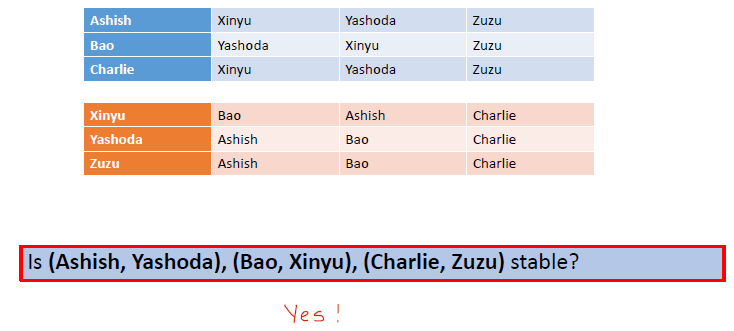
\includegraphics[width=0.5\linewidth]{stable_matching_example.png}
  	\end{tabular}
  	\begin{tabular}{l}
  		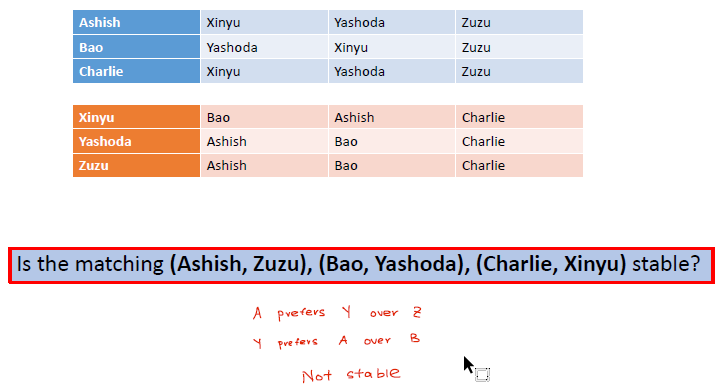
\includegraphics[width=0.5\linewidth]{stable_matching_bad.png}
  	\end{tabular}
  	\subsection{Gale‐Shapley Algorithm}
  	\begin{center}
  		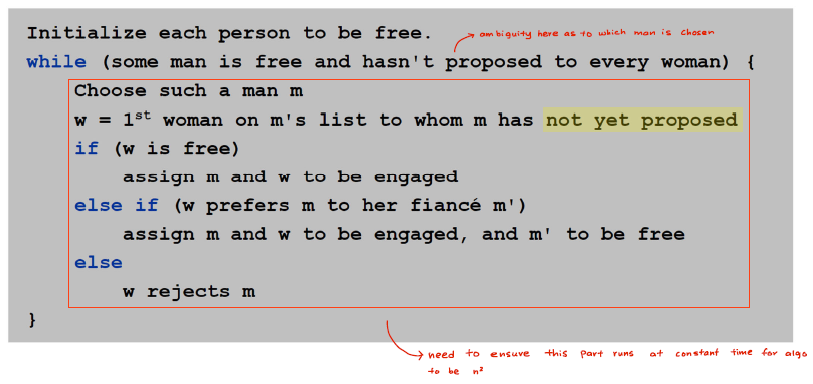
\includegraphics[width=0.9\columnwidth]{gale_shapley}
  	\end{center}
  	\subsubsection{Analysis of Gale-Shapley Algorithm}
  	\textbf{Lemma:} The \texttt{while} loop in Gale-Shapley runs in $\leq{n^2}$ time.\\\\
  	\textbf{Why?}
  	\begin{itemize}
  		\item A man never proposes to the same women twice when he makes a new proposal.
  		\item There are $n^2$ possible proposals, $\therefore$ there can only be $n^2$ loops
  		\item \textcolor{red}{Recurring idea in algorithm analysis: \textbf{Find a progress measure that keeps strictly increasing}, in this case its the \# of proposals}
  	\end{itemize}
	\subsubsection{Other general observation}
	\begin{itemize}
	  	\item Men propose to women in decreasing order of preference.
	  	\item Women's partners keep getting better.
	  	\item Each man is engaged to a unique woman.
	  	\item The matching produced is \textbf{stable}. Proof by contradiction:
	  	\begin{tightcenter}
	  		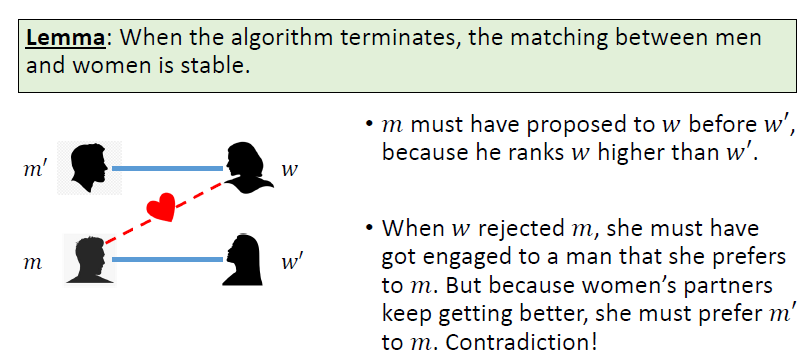
\includegraphics[width=0.7\columnwidth]{stable_output}
	  	\end{tightcenter}
  		\item The above version of Gale-Shapley produces \textit{man-optimal} stable matching where all man are matched with the $best(m)$
	\end{itemize}
	\subsubsection{Run time of Gale-Shapley Algorithm}
	Gale-Shapley Algorithm returns a \textbf{stable matching} in $O(N^2)$ time.
	\begin{itemize}
		\item Size of all preference profiles is $2n^2$, so cannot expect sub-quadratic running time, i.e. $O(N^2)$ is an optimal running time
	\end{itemize}
	\section{Asymptotic Analysis}
	\subsection{What is an Algorithm?}
	\begin{itemize}
		\item A \textcolor{red}{finite sequence} of \textcolor{red}{“well‐defined” instructions} to solve a given computational problem
	\end{itemize}
	\subsubsection{Objective}
	\begin{itemize}
		\item Design efficient algorithms in terms of:
		\begin{enumerate}         
			\item \textbf{Running tim}e, i.e. smallest $O(x)$
			\item Other matrix such as \textbf{space}
		\end{enumerate}
	\end{itemize}
	\subsection{How to analyze running time?}
	\begin{enumerate}         
		\item \textbf{Simulation}: Run the algorithm many times and measure the running time
		\begin{itemize}
			\item Tends to be \textbf{Machine Dependent} (different hardware) and \textbf{Input Dependent} (e.g. might work slow for $n=500$ but fast for $n=499$)
		\end{itemize}
		\item Mathematical Analysis
		\begin{itemize}
			\item Removes \textit{"external dependencies"} to give us a better idea of how fast algorithms run
		\end{itemize}
	\end{enumerate}
	\subsection{Word-RAM Model}
	\textbf{Assumptions}:
	\begin{itemize}
		\item Word is the basic storage of RAM which is basically a collection of bytes
		\item Any arbitrary location in RAM can be \textcolor{red}{accessed in the same time irrespective of location}
		\item Data as well as program \textcolor{red}{reside fully in RAM}
		\item Each arithmetic operation involves a \textcolor{red}{constant number of words} which takes a \textcolor{red}{constant number of CPU cycles} to run
	\end{itemize}
	\subsubsection{How to measure running time?}
	\begin{itemize}
		\item \textbf{Number of instructions executed} in the word-RAM Model
	\end{itemize}
	\begin{center}
		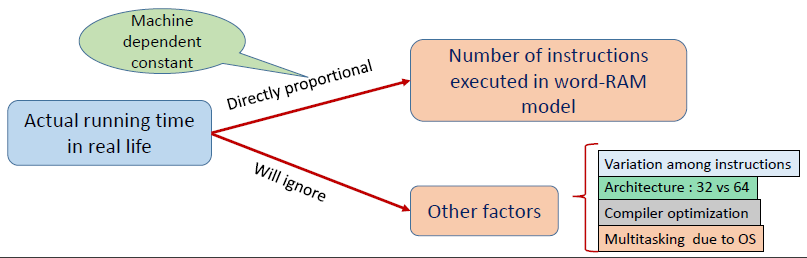
\includegraphics[width=0.67\columnwidth]{word_ram}
	\end{center}
	\subsection{Asymptotic Notations}
	\begin{center}
		\textbf{$O$-notation [upper bound ($\leq$)]: $f(n)=O(g(n))$\\}
		if $\exists c>0,n_0>0$ such that $\forall n\geq n_0$\\
		\fbox{$0\leq f(n)\leq cg(n)$}
		\ \\~\\ \textbf{$\Omega$-notation [lower bound ($\geq$)]: $f(n)=\Omega(g(n))$\\}
		if $\exists c>0,n_0>0$ such that $\forall n\geq n_0$\\
		\fbox{$0\leq cg(n)\leq f(n)$}
		\ \\~\\ \textbf{$\Theta$-notation [tight bound]: $f(n)=\Theta(g(n))$\\}
		if $\exists c_1,c_2,n_0>0$ such that $\forall n\geq n_0$\\
		\fbox{$0\leq c_1g(n)\leq f(n)\leq c_2g(n)$}
		\ \\~\\ \textbf{$o$-notation (<): $f(n)=o(g(n))$\\}
		if $\forall c>0,\exists n_0>0$ such that $\forall n\geq n_0$\\
		\fbox{$0\leq f(n)\leq cg(n)$}
		\ \\~\\ \textbf{$\omega$-notation (>): $f(n)=\omega(g(n))$\\}
		if $\forall c>0,\exists n_0>0$ such that $\forall n\geq n_0$\\
		\fbox{$0\leq cg(n)\leq f(n)$}
	\end{center}
	\ \\ \textcolor{red}{Note: $\Theta(g(n))=O(g(n))\cap{\Omega(g(n))}$}
	\subsection{Limits}
	Assume $f(n),g(n)>0$
	\begin{align*}
		&\lim\limits_{n \to \infty} \frac{f(n)}{g(n)} = 0 &\Rightarrow f(n) = o(g(n)) \\
		&\lim\limits_{n \to \infty} \frac{f(n)}{g(n)} < \infty &\Rightarrow f(n) = O(g(n)) \\
		0 < &\lim\limits_{n \to \infty} \frac{f(n)}{g(n)} < \infty &\Rightarrow f(n) = \Theta(g(n)) \\
		&\lim\limits_{n \to \infty} \frac{f(n)}{g(n)} > 0 &\Rightarrow f(n) = \Omega(g(n)) \\
		&\lim\limits_{n \to \infty} \frac{f(n)}{g(n)} = \infty &\Rightarrow f(n) = \omega(g(n))
	\end{align*}
	\begin{center}
		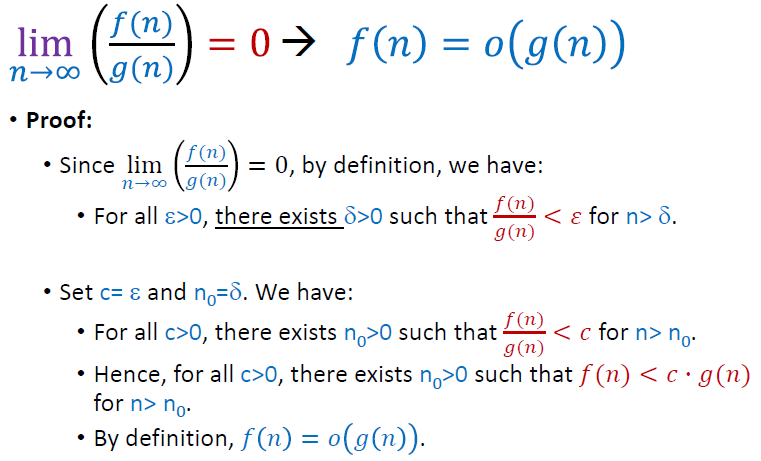
\includegraphics[width=0.7\columnwidth]{proof_delta_epsilon}
	\end{center}
	\subsection{Properties of Big-O}
	\begin{enumerate}
		\item \textbf{Transitivity}: applies for $O, \Theta, \Omega, o, \omega$
		\\ $f(n) = O(g(n)) \land g(n) = O(h(n)) \Rightarrow f(n) = O(h(n))$ 
		\item \textbf{Reflexivity}: for $O, \Omega, \Theta$ 
		\\ $\quad f(n) = O(f(n))$ 
		\item \textbf{Symmetry}: $f(n) = \Theta(g(n)) \iff g(n) = \Theta(f(n))$
		\item \textbf{Complementarity}: 
		\begin{itemize}
			\item $f(n) = O(g(n)) \iff g(n) = \Omega(f(n))$
			\item $f(n) = o(g(n)) \iff g(n) = \omega(f(n))$
		\end{itemize}
	\end{enumerate}
	\subsubsection{Common useful facts}
	\begin{itemize}
		\item if $f(n) = \omega(g(n))$, then $f(n) = \Omega(g(n))$
		\item if $f(n) = o(g(n))$, then $f(n) = O(g(n))$
		\item Degree-\textit{k} polynomials are $O(n^k)$.
		\item Degree-\textit{k} polynomials are $o(n^{k+1})$ and $\omega{(n^{k-1})}$.
		\item \textcolor{red}{Poly dominates logs:} $(\log{n})^{100}=o(n^{.0001})$, i.e. $n^k > (\log{n})^k$
		\item \textcolor{red}{Exponential dominate polys:} $n^{100}=o(2^{.001n})$, i.e. $2^{kn}>n^k$
		\item \hl{$1 < \log\log n < \log n < (\log n)^k < \sqrt{n} < n < n^k < a^n < n! < n^n$}
		\item $2^{2\cdot2^{\lg\lg n}}<n^2\lg\lg n<n^3\equiv\sum_{i=2}^{n}\dfrac{n^3}{i(i-1)}<n^{\lg n}<2^n<(\lg n)^n<n!$
	\end{itemize}
	\subsubsection{Common Confusions}
	\begin{itemize}
		\item $2^{n+5}=O(2^n)$, because $2^{n+5}=32\cdot{2^n}$
		\item \hl{$2^{5n}\neq O(2^n)$!!!}
		\item max($f(n),g(n)$) = $\Theta(f(n)+g(n))$, at most $f(n)+g(n)$, at least $1/2\times f(n)+g(n)$
		\item $\sin(n)\neq \Omega(\cos n)$
	\end{itemize}
	\subsubsection{Impossible combinations}
	\begin{itemize}
		\item $f(n)=\Omega(g(n))$ and $f(n)=o(g(n))$
		\item $f(n)=O(g(n))$ and $f(n)=\omega(g(n))$
	\end{itemize}
	
	\vfill\null\columnbreak
	
	\section{Iteration, Recursion and Divide-and-Conquer}
	\subsection{Iterative Algorithms}
	\begin{itemize}
		\item one or multiple loops $\rightarrow$ sequentially processing input elements
		\item \textbf{Loop invariant} implies correctness if
		\begin{itemize}
			\item \textit{\textbf{Initialization}}: invariant is true before first iteration of loop
			\item \textit{\textbf{Maintenance}}: if invariant is true before an iteration, it remains true at beginning of next iteration
			\item \textit{\textbf{Termination}}: invariant provides a useful property for showing correctness when program terminates
		\end{itemize}
		\item Examples
		\begin{itemize}
			\item InsertionSort: subarray $A[1...j-1]$ consists of elements originally in $A[1...j-1]$ but in sorted order
			\item SelectionSort: subarray $A[1...j-1]$ is sorted and contains the $j-1$ smallest elements of $A$
		\end{itemize}
	\end{itemize}
	\subsection{Divide-and-Conquer}
	Consists of 3 parts:
	\begin{enumerate}         
		\item \textit{\textbf{Divide}} problem into smaller subproblems 
		\item \textit{\textbf{Conquer}} subproblems by solving recursively, small subproblems are trivial to solve
		\item \textit{\textbf{Combine}} solutions of subproblems into solution of original problem
	\end{enumerate}
	\subsubsection{Tower of Hanoi}
	\begin{center}
		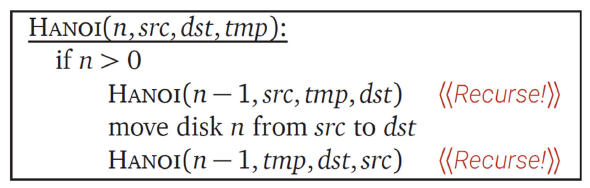
\includegraphics[width=0.7\columnwidth]{tower_of_hanoi}
	\end{center}
	\begin{itemize}
		\item Runtime: $T(n)=2\cdot T(n-1)+1=2^n-1$
	\end{itemize}
	\subsubsection{Merge Sort}
	$T(n) = \begin{cases}
		\Theta(1)  & if n = 1 \\
		2T(\dfrac{n}{2})+\Theta(n) & if n > 1
	\end{cases}$ 
	\\ Running time: $\Theta(n\lg n)$
	\subsection{How to solve recurrence?}
	Recurrence equation typically comes in the form \[T(n)=aT(n/b)+f(n)\]where $a$ is the \# of subproblems, $n/b$ is the subproblem size and $f(n)$ is the time to divide and combine
	\subsubsection{Recursion Tree}
	Running time = height of tree $\times$ number of leaves
	\begin{itemize}
		\item Each node represents cost of a single subproblem
		\item Height of tree = longest path from root to leaf
	\end{itemize}
	\begin{tabular}{l}
		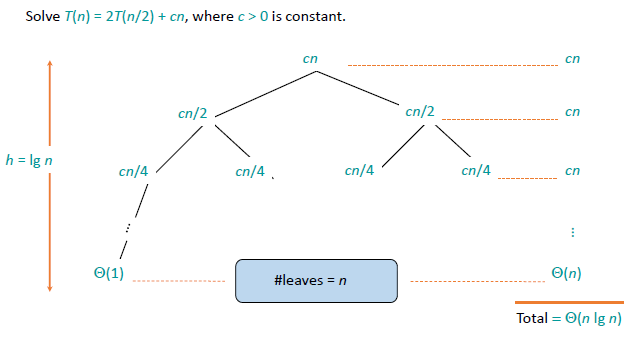
\includegraphics[width=0.45\linewidth]{recursion_tree_1}
	\end{tabular}
	\begin{tabular}{l}
		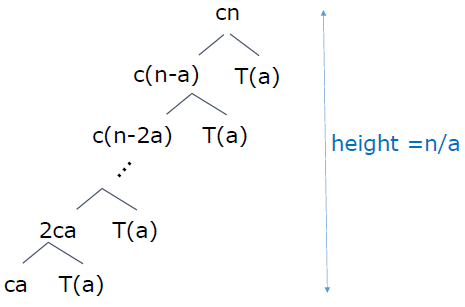
\includegraphics[width=0.45\linewidth]{recursion_tree_2}
	\end{tabular}
	\subsubsection{Master Method}
	\begin{math}
		T(n) = aT(\frac{n}{b}) + f(n) = \begin{cases}
			\Theta(n^{\log_ba}) & \text{ if } f(n) < n^{\log_ba} \text{ polynomially}
			\\ \Theta(n^{\log_ba} \log n) & \text{ if } f(n) = n^{\log_ba} 
			\\ \Theta(f(n)) & \text{ if } f(n) > n^{\log_ba} \text{ polynomially}
		\end{cases}
	\end{math} 
	where $a\geq 1, b>1$ and $f$ is asymptotically positive
	\textbf{3 common cases of Master Method}
	\begin{enumerate}
		\item If $f(n) = O(n^{\log_b a-\varepsilon})$ for some constant  $\varepsilon > 0$, 
		\begin{itemize}
			\item $f(n)$ grows polynomially slower than $n^{\log_ba}$ by $n^\varepsilon$ factor.
			\item then $T(n) = \Theta(n^{\log_ba})$.
		\end{itemize}
		\item If $f(n) = \Theta(n^{\log_ba} \log^kn) $ for some $k \geq 0$,
		\begin{itemize}
			\item $f(n)$ and $n^{\log_ba}$ grow at similar rates.
			\item then $T(n) = \Theta(n^{\log_ba}\log^{k+1} n)$
		\end{itemize}
		\item If $f(n) = \Omega(n^{\log_ba + \varepsilon})$ for some constant $\varepsilon > 0$, 
		\begin{itemize}
			\item and $f(n)$ satisfies the \textbf{regularity condition} 
			\begin{itemize}
				\item $af(n/b) \leq cf(n)$ for some constant $c<1$ and all sufficiently large $n$
				\item this guarantees that the sum of subproblems is smaller than $f(n)$.
			\end{itemize} 
			\item $f(n)$ grows polynomially faster than $n^{\log_ba}$ by $n^\varepsilon$ factor
			\item then $T(n) = \Theta(f(n))$.
		\end{itemize}
	\end{enumerate}
	\captionof*{table}{Examples of Master Theorem Cases}
	\begin{tabular}{l}
		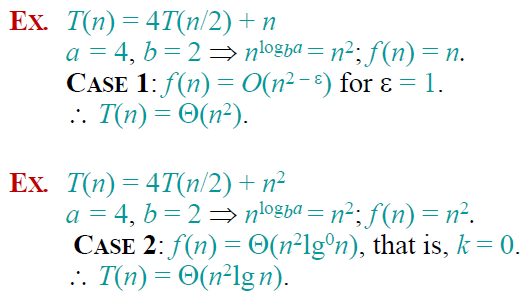
\includegraphics[width=0.45\linewidth]{master_theorem_1}
	\end{tabular}
	\begin{tabular}{l}
		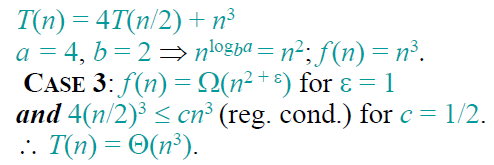
\includegraphics[width=0.45\linewidth]{master_theorem_2}
	\end{tabular}
	\captionof*{table}{Examples where Master Theorem Don't Work}
	\begin{tabular}{l}
		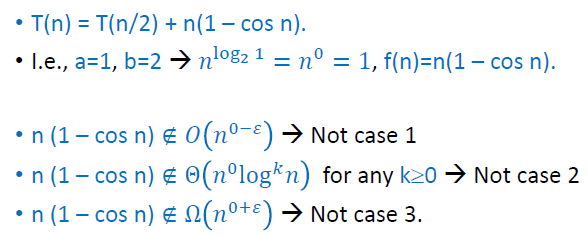
\includegraphics[width=0.45\linewidth]{wrong_master_theorem_1}
	\end{tabular}
	\begin{tabular}{l}
		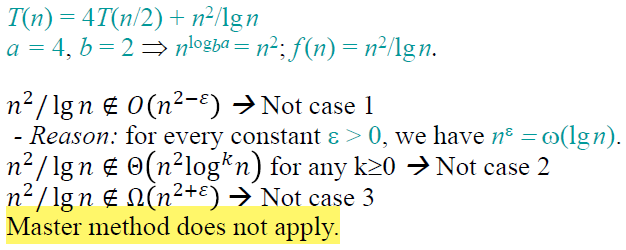
\includegraphics[width=0.45\linewidth]{wrong_master_theorem_2}
	\end{tabular}
	\subsubsection{Substitution Method}
	\begin{enumerate}
		\item guess that $T(n) = O(f(n))$. 
		\item verify by induction:
		\begin{enumerate}
			\item to show that for $n \geq n_0$, $T(n) \leq c \cdot f(n)$
			\item set $c = \max\{2, q\}$ and $n_0 = 1$
			\item verify base case(s): $T(n_0) = q$
			\item recursive case ($n > n_0$):
			\begin{itemize}
				\item by strong induction, assume $T(k) \leq c \cdot f(k)$ for $n > k \geq n_0$
				\item T(n) = <recurrence> ... $\leq c \cdot f(n)$
			\end{itemize}
			\item hence $T(n) = O(f(n))$.
		\end{enumerate}
	\end{enumerate}
	\textcolor{red}{Note that this may not be a tight bound!}
	\\ \textbf{Example}
	\\ $T(n)=4T(n/2)+n$
	\begin{enumerate}         
		\item Assume $T(1)=q$, where $q$ is a constant
		\item Show that for $n\geq n_0$, $T(n)\leq c_1n^2-c_2n$
		\item Set $c_1=q+1$ and $c_2=1$ and $n_0=1$
		\item \underline{Base case} ($n=1$): $T(1)=q\leq (q+1) (1)^2-(1)(1)$
		\item \underline{Recursive case} ($n>1$): 
		\begin{itemize}
			\item By strong induction: assume $T(k)\leq c_1\cdot k^2-c_2\cdot k$ for $n>k\geq 1$
			\item $T(n)=4T(n/2)+n=4(c_1(n/2)^2-c_2(n/2))+n=c_1n^2-2c_2n+n
			\\\null\quad\qquad=c_1n^2-c_2n+(1-c_2)n$
			\item Since $(1-c_2)=0,T(n)\leq c_1n^2-c_2n$
		\end{itemize}
	\end{enumerate}
	\section{Randomized Algorithm}
	\subsection{Random Variables and Expectation}
	\begin{itemize}
		\item A discrete random variable is a function from a sample space to the integers
		\item Expectation: $\mathbb{E}[X]=\sum_ii\cdot \Pr[X=i]$
		\item Linearity of Expectations: $\mathbb{E}[X+Y]=\mathbb{E}[X] + \mathbb{E}[Y]$ for any 2 random variable $ X $ and $ Y $ and $ \mathbb{E}[aX]=a\mathbb{E}[X] $
	\end{itemize}
	\subsection{Quicksort}
	\begin{itemize}
		\item Divide-and-conquer Algorithm with linear time $ \Theta(n) $ partitioning subroutine
		\item Suppose the pivot produces subarrays of size $ j $ and $ (n-j-1) \rightarrow T(n)=T(j)+T(n-j-1)+\Theta(n) $ 
		\item Worst case will occur when we select the first element of a sorted array as pivot \[ T(n)=T(0)+T(n-1)+\Theta(n)\Rightarrow\Theta(n^2) \]
	\end{itemize}
	\subsubsection{Average Case Analysis of Quicksort}
	\begin{proof}
		for quicksort, $A(n) = O(n \log n)$
		
		Let $P(i)$ be the set of all those permutations of elements $\{e_1, e_2, \dots, e_n\}$ that begins with $e_i$.
		
		Let $G(n, i)$ be the average running time of quicksort over $P(i)$.
		Then $G(n) = A(i-1) + A(n-i) + (n-1)$, where
		$A(n) = \frac{1}{n} \sum_{i=1}^n G(n, i)$
		\\ $\qquad = \frac{1}{n} \sum_{i=1}^n ( A(i-1) + A(n-i) + (n-1) )$
		\\ $\qquad = \frac{2}{n} \sum_{i=1}^n A(i-1)+n-1$
		\\ $\qquad = O(n\log n)$ by taking it as area under integration
	\end{proof}
	\subsubsection{Quicksort vs Mergesort}
	\begin{center}
		\begin{tabular}{|c|c|c|c|}
			\hline
			& Average & Best & Worst \\\hline
			Quicksort & $1.39n\lg n$ &  $n \lg n$ & $n(n-1)$ \\\hline
			Mergesort & $n\lg n$ &  $n \lg n$ & $n \lg n$ \\\hline
		\end{tabular}
	\end{center}
	\begin{itemize}
		\item Disadvantages of MergeSort:
		\begin{itemize}
			\item overhead of temporary storage
			\item cache misses
		\end{itemize}
		\item Advantages of QuickSort
		\begin{itemize}
			\item in place
			\item reliable (as $n \uparrow$, chances of deviation from avg case $\downarrow$)
		\end{itemize}
		\item Issues with quicksort
		\begin{itemize}
			\item \textcolor{red}{distribution-sensitive} time taken depends on the initial (input) permutation
		\end{itemize}
	\end{itemize}
	\subsection{Randomized Algorithm}
	\subsubsection{Randomized vs Non-Randomized}
	\begin{itemize}
		\item Randomized: output and running time are \textbf{functions of the input and random bits chosen}
		\item Non-Randomized: output \& running time are functions of the input only
	\end{itemize}
	\subsubsection{Types of Randomized Algorithms}
	\begin{enumerate}         
		\item Randomized \textcolor{red}{Las Vegas} Algorithm:
		\begin{itemize}
			\item Output is \textbf{always correct} (e.g. Randomized QuickSort)
			\item Running time is a random variable
		\end{itemize} 
		\item Randomized \textcolor{red}{Monte Carlo} Algorithm
		\begin{itemize}
			\item \textbf{Output may be incorrect} with small probability
			\item Running time is deterministic
		\end{itemize}
	\end{enumerate}
	\subsubsection{Randomized Quicksort}
	\begin{itemize}
		\item Choose random pivot 
		\item Probability that the run time of Randomized Quick Sort exceeds average by $ x\%=n^{-\dfrac{x}{100}\ln\ln n} $
		\item P(run time of randomized quicksort is double average) = $10^{-15}$ for $n\geq 10^6$
	\end{itemize}
	\subsubsection{Analysis of Randomized Quicksort}
	\begin{enumerate}         
		\item Let $ T_\pi $ be the number of comparisons made by the algorithm when the input permutation is $\pi$. $ T_\pi $ is a random variable.
		\\ $ T_\pi=n-1+T_{\pi_l}+T_{\pi_r} $ where $ n-1 $ is the partition algorithm, $\pi_l$ and $\pi_r$ are the left and right parts of the partition 
		\begin{itemize}
			\item Note that the left and right partition are of random length due to the random choice of the pivot
		\end{itemize}
		\item $ \mathbb{E}[T_{\pi_l}+T_{\pi_r}]=\dfrac{1}{n}\sum\limits_{i=1}^{n}\mathbb{E}[T_{\pi_l}|q=i]+\mathbb{E}[T_{\pi_r}|q=i] $
		$\leq\dfrac{1}{n}\sum\limits_{i=1}^{n}E(i-1)+E(n-i)$
		\item $ E(n)\leq n-1 + \dfrac{1}{n}\sum\limits_{i=1}^{n}E(i-1)+E(n-i)=n-1+\dfrac{2}{n}\sum\limits_{i=1}^{n-1}E(i)=O(n\lg n) $
		\item Very high probability that randomized quick sort will run in $n\lg n$ time which is the case for the average-case quicksort!
	\end{enumerate}
	\section{Hashing}
	\subsection{Dictionary Data Structure}
	\begin{itemize}
		\item 3 different types:
		\begin{itemize}
			\item \textbf{Static}: fixed set of inserted items fixed; only care about queries
			\item \textbf{Insertion-only}: only insertions and queries
			\item \textbf{Dynamic}: insertions, deletion and queries
		\end{itemize}
		\item Implementations
		\begin{itemize}
			\item \textbf{sorted list} (static) - Query takes $ O(\log n)$ using binary search
			\item \textbf{balanced search Trees} (dynamic) - $ O(\log n) $ for all operations
			\item \textbf{Direct Access Table}
			\begin{itemize}
				\item Needs items to be represented as non-negative numbers (i.e. prehashing required)
				\item \textcolor{red}{Huge space requirement} (same as universe size)
				\item Operations are all $ O(1) $
			\end{itemize}
		\end{itemize}
	\end{itemize}
	\subsection{Hashing}
	\begin{itemize}
		\item \textbf{Hash function}: $ h: U \rightarrow \{1,...,M\} $ gives the location of where to store in hash table. Basically maps the universe into 1 of M buckets
		\item \textbf{Collision}: for 2 different keys $ x,y $, $ h(x)=h(y) $
		\begin{itemize}
			\item Resolve collisions by using \textbf{chaining, open addressing} etc.
		\end{itemize}
		\item \textbf{Desired Properties}:
		\begin{itemize}
			\item \checkmark minimise collisions - \codeblue{query(x)} and \codeblue{delete(x)} take $\Theta(|h(x)|)$. Worst case is when all keys hash to the same location in which case operations will take $\Theta(N)$ time
			\item \checkmark minimuse storage space - aim to have $ M=O(N) $, where $N$ is the \# of stored items
			\item \checkmark function $ h $ is easy to compute - assume $ h(x) $ runs at constant time
		\end{itemize}
		\item If $ |U|\geq (N-1)M+1 $, for any $ h:U\rightarrow[M] $, there is a set of N elements having the same hash value
		\begin{itemize}
			\item Proof (\textit{pigeonhole principle}): If every slot in hashtable had $ <N $ elements, then $ |U|\leq(N-1)M $ which is a contradiction. 
		\end{itemize}
	\end{itemize}
	\subsection{Randomization}
	To prevent adversary, we randomize the hash function!
	\subsubsection{Universal Hashing}
	Suppose $\mathcal{H}$ is a set of hash functions mapping $U$ to $[M]$. 
	\begin{center}
		$ \mathcal{H} $ is universal if $\forall x\neq y$: $\dfrac{|h\in\mathcal{H}:h(x)=h(y)|}{|\mathcal{H}|}\leq \dfrac{1}{M}$ \\ OR $\Pr\limits_{h\sim\mathcal{H}}[h(x)=h(y)]\leq \dfrac{1}{M}$
	\end{center}
	\textbf{Examples:}
	\begin{center}
		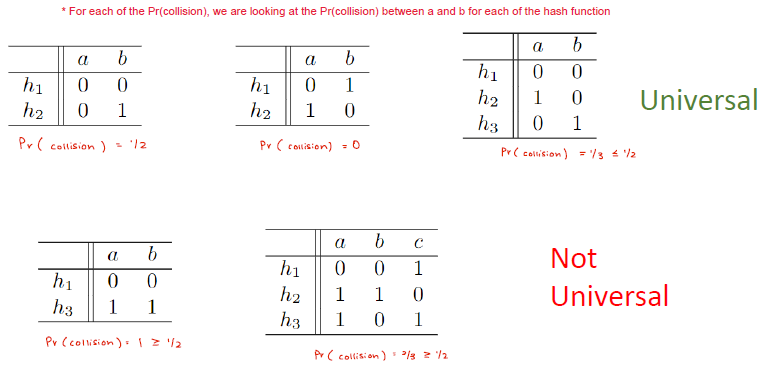
\includegraphics[width=0.8\columnwidth]{universal_hashing}
	\end{center}
	\begin{itemize}
		\item For a single, \textit{deterministic}, hash function from a universal family $\mathcal{H}$, if $x,y$ are chosen uniformly from universe $U$, the probability of $h(x)=h(y)=1$. e.g. In all-zero function, everything will map to 0
		\item It is \textcolor{red}{possible for a uniform family of hash function to NOT be universal}. e.g. Let $h_i$ be the hash function that maps all of $U$ to $i$. Then ${h_1,...,h_i}$ is uniform but not universal
	\end{itemize}
	\subsubsection{Collision Analysis for Universal family of hash}
	\textbf{Claim}: For any $N$ elements $x_1,...,x_N$, the expected number of collisions between $x_N$ and the other elements is $<\dfrac{N}{M}$
	\\ \textbf{Proof}
	\begin{enumerate}         
		\item For $i<N$, let $A_i=1$ if $h(x_i)=h(x_n)$ and 0 otherwise
		\item $\mathbb{E}[A_i]=1\cdot\Pr[A_i=1]+0\cdot\Pr[A_i=1]\leq \dfrac{1}{M} $
		\item \# of collisions with $x_N$ is $\sum_{i<N}A_i$
		\item $\mathbb{E}[\sum_{i<N}A_i]=\sum_{i<N}\mathbb{E}[A_i]\leq(N-1)/M$
	\end{enumerate}
	\begin{itemize}
		\item From the claim above, each operation will hence cost $O(1)$ in expectation and by linearity of expectations, total cost of $N$ inserts will be $ O(N) $
	\end{itemize}
	\subsubsection{Construction of universal family}
	\begin{itemize}
		\item Supposed $U$ is indexed by $ u $-bit strings, and $ M=2^m $. For any binary matrix $ A $ with $ m $ rows and $ u $ columns: $h_A(x)=Ax(\text{mod}2)$
		\begin{itemize}
			\item $ x $ is a $ u\times1 $ matrix $\Rightarrow$ $ Ax $ is $ m\times1 $
		\end{itemize}
		\item Suppose $ U={00,01,10,11} $ and $ M=2 $.
		\\*
		\begin{tightcenter}
			{\rowcolors{2}{gray!15}{gray!5}
			\begin{tabular}
				{ccccc}
				\rowcolor{cyan!10} 
				\hline
				\, & 00 & 01 & 10 & 11 \\\hline
				$h_{00}$ & 0 & 0 & 0 & 0 \\
				$h_{01}$ & 0 & 1 & 0 & 1 \\
				$h_{10}$ & 0 & 0 & 1 & 1 \\
				$h_{11}$ & 0 & 1 & 1 & 0 \\\hline
			\end{tabular}
			}
		\end{tightcenter} 
		\item In this case, $u=2$ since it is a 2-bit string, $m=1$, $A=\{[0,0], [0,1], [1,0], [1,1]\}$
	\end{itemize}
	\vfill\null\columnbreak
	\textbf{Proof}
	\begin{itemize}
		\item Let $x\neq y$ and $z=x-y$. We know that $z\neq 0$.
		\item We want to show that the probability of collision, i.e. $\Pr\limits_{A}[Ax=Ay] = \Pr\limits_{A}[A(x-y)=0]=\Pr\limits_{A}[Az=0]\leq \dfrac{1}{M}$ 
		\item Suppose $z$ is 1 at the $i^{th}$ coordinate and 0 everywhere else. Then $Az$ equals the $i^{th}$ column of $A$. Since the columns are uniformly random, $\Pr[Az=0]=\dfrac{1}{2^m}=\dfrac{1}{M}$ (probability that every element in the $i^{th}$ column is 0)
	\end{itemize}
	\textbf{Additional Notes}:
	\begin{itemize}
		\item In addition to storing the Hash table, using the matrix method will need to store the matrix $A$.
		\begin{itemize}
			\item Addtional storage overhead of $\Theta(\log N\cdot \log U)$ bits, if $M=\Theta(N)$
		\end{itemize}
	\end{itemize}
	\subsection{Perfect Hashing}
	\begin{itemize}
		\item \textbf{Static Case}: $N$ fixed items in dictionary, $x_1,x_2,...,x_N$. Want to perform \texttt{Query} in $O(1)$ time
		\item Possible to do it by using \textbf{Quadratic Space}, i.e. $M=N^2$
	\end{itemize}
	\textbf{Claim}: If $\mathcal{H}$ is universal and $M=N^2$, then if $h$ is sampled uniformly from $\mathcal{H}$, expected number of collision is $<1$
	\\ \textbf{Proof}:
	\begin{itemize}
		\item For $i\neq j$, let $A_{ij}=1$ if $h(x_i)=h(x_j)$ and 0 otherwise
		\item By universality, $\mathbb{E}[A_{ij}]=\Pr[A_{ij}=1]\leq \dfrac{1}{M}=\dfrac{1}{N^2}$
		\item $\mathbb{E}[\#c\text{collisions}]=\sum_{i\neq j}\mathbb{E}[A_{ij}]\leq {N\choose 2}\dfrac{1}{N^2}<1$
	\end{itemize}
	\subsubsection{2-level Scheme}
	\begin{itemize}
		\item Choose $h:U\rightarrow[N]$ from a universal hash family
		\item Let $L_k$ be the number of $x_i$'s for which $h(x_i)=k$, i.e. $L_k$ is the number of elements from $U$ that all maps to a bucket $k\in N$ 
		\item Choose $h_1,...,h_N$ \textcolor{red}{second-level} hash functions $h_k:[N]\rightarrow[L_k^2]$ such that there are no collisions among the $L_k$ elements mapped to $k$ by $h$ 
	\end{itemize}
	\captionof*{figure}{Example of 2-Level Scheme}
	\begin{center}
		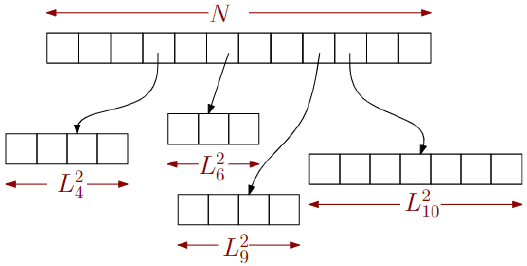
\includegraphics[width=0.5\columnwidth]{2_level_hash}
	\end{center}
	\textbf{Claim}: If $\mathcal{H}$ is universal, then if $h$ is sampled uniformly:
	\[\mathbb{E}\left[\sum\limits_{k}L_k^2\right]<2N\]
	\textbf{Proof}:
	\begin{itemize}
		\item For $1\leq i, j\leq N$, define $A_{ij}=1$ if $h(x_i)=h(x_j)$ and $A_{ij}=0$ otherwise
		\item \textbf{Crucial Observation}: $\sum\limits_{k}L_k^2=\sum\limits_{i,j}A_{ij}$
		\item $\mathbb{E}[\sum_{ij}A_{ij}]=\sum_i[A_{ii}]+\sum_{i\neq j}\mathbb{E}[A_{ij}]\leq N\cdot 1 + N(N-1)\cdot(\dfrac{1}{N})<2N$
	\end{itemize}
	\section{Amortized Analysis}
	\begin{itemize}
		\item \textbf{Amortized analysis} guarantees the \textit{average} performance of each operation in the \textit{worst case}
		\item It is a strategy for analysing a \textcolor{red}{sequence of operations} to show the average cost of operation is small even tho a single operation within the sequence might be expensive
		\begin{itemize}
			\item Note that in Amortized Analysis, there are \textbf{no randomness involved} and is \textbf{only used for deterministic algorithm}
			\item \textcolor{red}{DO NOT} get confused with average-case analysis which is used for random input
			\item \textcolor{red}{DO NOT} get confused with expected run time which is used for probabilistic algorithms
		\end{itemize}  
		\item Total amortized cost provides an \textit{upper bound} on the total true cost
	\end{itemize}
	\subsection{Types of Amortized Analysis}
	\subsubsection{Aggregate Method}
	\begin{itemize}
		\item look at the whole sequence, sum up the cost of operations and take the average - simple but lacks precision
		\item e.g. binary counter - amortized $O(1)$
		\item e.g. queues (with \texttt{INSERT} and \texttt{EMPTY}) - amortized $O(1)$
	\end{itemize}
	\subsubsection{Accounting Method}
	\begin{itemize}
		\item Charge $i^{th}$ operation a fictitious amortized cost $c(i)$
		\item Idea is that amortized cost $c(i)$ is a \textcolor{red}{fixed cost for each operation}, whereas true cost $t(i)$ varies depending on when operation is called
		\item Amortized cost $c(i)$ must satisfy:
		\[\sum_{i=1}^{n}t(i)\leq\sum_{i=1}^{n}c(i) \text{ for all } n\] 
		\item Typically fixed amortized cost $c(i)$ will be more than true cost $t(i)$. 
		\item Extra amount we pay for cheap operation can be use to pay for the expensive operation
		\begin{itemize}
			\item \textbf{Invariant}: Bank account is always > 0
		\end{itemize}
		\item \textcolor{red}{NOTE}: Different operations can have different amortized costs.
	\end{itemize}
	\textbf{Example: Queues}
	\begin{itemize}
		\item \texttt{INSERT} have amortized cost of 2 (true cost of 1)
		\item \texttt{EMPTY} have amortized 0 (true cost is size of queue)
		\item Whenever an element is inserted, we pay 1 extra to be used for deleting it later
		\item Total cost is at most 2*\#INSERT $\leq$ 2$n$
	\end{itemize}
	\vfill\null\columnbreak
	\subsubsection{Potential Method}
	\begin{itemize}
		\item $\phi$: Potential function associated with algorithm/data structure
		\item $\phi(i)$: Potential at the $i^{th}$ operation
		\item Important condition to be fulfilled by $\phi$: $\phi(i)\geq 0$ for all $i$
		\item Amortized cost of $i$th operation $\stackrel{\text{def}}{=}$ True cost of $i$th operation + $\Delta\phi_i$
		\item Typically, $\phi(0) = 0$
		\item To find for a suitable $\phi$, try to find something that \textcolor{red}{decrease during the costly operation}
	\end{itemize}
	\textbf{Example: Binary Counter}
	\begin{itemize}
		\item Actual cost of $i$th operation = 1 + Length of longest suffix with all 1's
		\item $\phi(i)$: Number of 1's in the counter after the $i$th increment
		\begin{tabular}{|c|c|c|}
			\hline
			True $i$th increment & $\Delta\phi_i$ & Amortized cost of $i$th increment \\\hline
			$l_i+1$ & $-l_i+1$ & $2$ \\\hline
		\end{tabular}
		\item Amortized cost of $n$ increments $=2n=O(n)$ \textbf{ if starting from all 0s}
		\item Amortized cost of $n$ increments $\leq O(n+t)$ \textbf{if starting from $t$ 1s}
	\end{itemize}
	
	\section{Miscellaneous}
	\subsection{Useful Facts}
	\begin{multicols*}{2}
		\begin{itemize}
			\item $e^x\geq 1+x$
			\item $ (1-\dfrac{1}{n})^n\approx\dfrac{1}{e} $
			\item $\sum\limits_{j=0}^{\lg(n-1)}2^j=2^{\lg(n-1)+1}-1\\ \hspace*{4em}\leq{2(n-1)}$
			\item $a=b^{\log_ba}$
			\item $\log_c(ab)=\log_ca+\log_cb$
			\item $\sum\limits^{\lg n}_{i=0}\dfrac{1}{\lg n/{a^i}} = \lg\lg n$
			\item $(\lg n)!\leq \lg n^{\lg n}=2^{\lg n \lg\lg n}$
			\item $\sum_{i=1}^{\lg n}\lg\lg \frac{n}{i}=\lg n\lg\lg n$
			\item $\log_ba^n=n\log_ba$
			\item $\log_ba=\dfrac{\log_ca}{\log_cb}$
			\item $\log_b(1/a)=-\log_ba$
			\item $\log_ba=\dfrac{1}{\log_ab}$
			\item $a^{\log_bc}=c^{\log_ba}$
			\item $\dfrac{d}{dn}\lg\lg n = \dfrac{1}{n\lg n}$
			\item $n^2\log_nn!=n^2\times \frac{\lg n!}{\lg n}=n^3$
		\end{itemize}
	\end{multicols*}
	
	\subsection{Approximations and Series}
	\begin{itemize}
		\item Stirling's Approximation:
		\begin{itemize}
			\item $n!=\sqrt{2\pi n}(\dfrac{n}{e})^n(1+\Theta(\dfrac{1}{n}))$
			\item $\log(n!)=\Theta(n\log n)$
		\end{itemize}
		\item Arithmetic Series: $\sum_{k=1}^n=1+2+3+\cdots+n=\dfrac{1}{2}n(n+1)=\Theta(n^2)$
		\item Harmonic Series: $\sum^n_{k=1}\dfrac{1}{k}=\Theta(\lg(n))$
		\item Geometric Series: $\sum_{k=0}^nx^k=1+x+x^2+\cdots+x^n=\dfrac{x^{n+1}-1}{x-1}$
		\item Geometric Series: $\sum_{k=0}^\infty x^k=\dfrac{1}{1-x}$ when $|x| < 1$
		\item L'Hopital's Rule: $\lim\limits_{x \to \infty}\dfrac{f(x)}{g(x)}=\lim\limits_{x \to \infty}\dfrac{f'(x)}{g'(x)}$
	\end{itemize}
	\subsubsection{Arithmetic and Geometric Series}
	\begin{center}
		\begin{tabular}{|c|c|c|}
			\hline
			& Arithmetic & Geometric \\\hline
			$a_n$ & $a_n=a_1+d(n-1)$ & $a_n=a_1\cdot r^{n-1}$ \\\hline
			$S_n$ & $S_n=\dfrac{n}{2}(a_1+a_n)$ & $S_n=a_1\left(\dfrac{1-r^n}{1-r}\right)$ \\\hline
			Infinite Series & & $S_\infty=\dfrac{a_1}{1-r}$, |$r$| < 1 \\\hline
		\end{tabular}
	\end{center}
	\subsection{Permutations and Combinations}
	\begin{itemize}
		\item nPr = n! / (n-r)!
		\item nCr = n! / (n-r)!r!
		\item $\binom{2n}{n}\approx2^{2n}/\sqrt{n}$
	\end{itemize}
	\subsection{Coupon Collector Problem}
	\begin{itemize}
		\item There are $n$ types of coupon given out by the store
		\item Each time you visit the store you get 1 ticket at random
		\item What is the expected number of visits before you collect at least one of each type of coupon
		\item Pr(new coupon collected) = $\left(\dfrac{n-(i-1)}{n}\right)$
		\item Let $T_i$ be the \# of trials before success
		\item $\mathbb{E}[T_1+T_2+...+T_n] = \mathbb{E}[T_1] + \mathbb{E}[T_2] + ... + \mathbb{E}[T_n] = n/n + n/(n-1) + ... + n/(n-(n-1)) = n (1+1/2+...+1/n)=O(n\lg n)$
	\end{itemize}
	\subsection{$n$ bins $n$ balls problem}
	Suppose that you throw $n$ balls uniformly and independently at random into $n$ bins. What does the expected fraction of bins with exactly 3 balls converge to as $n\rightarrow\infty$
	\begin{itemize}
		\item Pr[ball go into bin $k$] = $\dfrac{1}{n}$, Pr[ball goes into any other bin] = $1-\dfrac{1}{n}$
		$\begin{aligned} 
			\text{Pr[3 balls go into 1 bin]} &= \binom{n}{3}(\dfrac{1}{n^3})(1-\dfrac{1}{n})^{n-3} \\ 
			&= \dfrac{n(n-2)}{6(n-1)^2}(1-(1/n))^n \\
		\end{aligned}$
		\item $(1-\dfrac{1}{n})^n\approx\dfrac{1}{e}$, $\lim_{n\rightarrow\infty}\dfrac{n(n-2)}{6(n-1)^2}=1/6$, limit = $\dfrac{1}{6e}$
	\end{itemize}
	\vfill\null\columnbreak
	\subsection{Potentially useful algos}
	\subsubsection{Karp Rabin (find substrings)}
	\begin{itemize}
		\item Given a text \texttt{txt[0...n-1]} and a pattern \texttt{pat[0...m-1]}, write a function \texttt{search} that prints all occurrences of pat[] in txt[]. You may assume that n > m.
		\item Idea is that you can hash the patterns as well as substrings in original array so that you can efficiently find the patterns in the array without having to manually loop through each element and then checking whether it matches the pattern
		\item Let the length of each pattern be $k$. Runtime will be $O(nk + mk)$.
	\end{itemize}
	\subsection{Adversarial Argument}
	\subsubsection{Merge needs $2n-1$ comparisons}
	\textbf{Question}: Give an adversarial argument to show that at least $2n-1$ comparisons are needed to merge two sorted arrays $A = [A1,A2,...,An]$ and $B = [B1,B2, ...,Bn]$ into one sorted array by any comparison-based algorithm.
	\begin{enumerate}
		\item Take $A=[1,3,5,...,2n-1],B=[2,4,6,...,2n]$
		\item Suppose $\mathcal{M}$ outputs the correct sorted array $[1,2,...,2n-1,2n]$ where $\mathcal{M}$ makes $<2n-1$ comparisons
		\item There must exist 2 consecutive elements in the error that were never compared, 1 element from $A$ and 1 element from $B$
		\item Suppose "3" and "4" were the ones not compared
		\item Set $A'=A,B'=[2,2.99,6,...,2n]$, where 4 is replaced by 2.99.
		\item We know that "3" in $A$ and 2.99 in $B$ will not be compared and thus
		$\mathcal{M}$ will output $[1,2,3,2.99,5,...,2n-1,2n]$
		\item Therefore must have $2n-1$ comparisons
	\end{enumerate}
\end{multicols*}
\end{document}
